\documentclass[aspectratio=169,xcolor={dvipsnames}
,hide notes
%,show only notes
%,show notes on second screen=right
]{beamer}
\usetheme[background=light, numbering=fraction]{metropolis}
\usepackage{appendixnumberbeamer}

\usepackage[labelfont=bf,textfont={it}]{caption}
\usepackage{subcaption}
\captionsetup[figure]{justification=centering}
\captionsetup[subfigure]{justification=centering}

%\usepackage{fontspec}
%\setsansfont{Fira Sans Mono}

\usepackage[binary-units]{siunitx}
\sisetup{range-phrase=--, range-units=single}

\usepackage[UKenglish]{babel}
\usepackage{csquotes}

\usepackage{amssymb}

\usepackage{lipsum}
\usepackage[basic]{complexity}
\usepackage[super,negative]{nth}

\usepackage{booktabs}

%bib
\usepackage[maxnames=3,maxbibnames=99,mincrossrefs=5,sortcites
,backend=bibtex
,style=authortitle
]{biblatex}
\addbibresource{papers-off.bib}
\addbibresource{confs-off.bib}
\addbibresource{books-off.bib}
\addbibresource{rfc.bib}
\addbibresource{misc.bib}

%picky abt et al.
\usepackage{xpatch}

\xpatchbibmacro{name:andothers}{%
	\bibstring{andothers}%
}{%
	\bibstring[\emph]{andothers}%
}{}{}

%opening!

\usepackage{cleveref}
\newcommand{\crefrangeconjunction}{--}

\usepackage{fontawesome}

%-------------------------------------%
%-------------------------------------%

\title{Reinforcement Learning in Network Defence/Control (WIP)}
\author{Kyle A. Simpson\\
	\small{\faGithub{} \href{https://github.com/felixmcfelix}{FelixMcFelix} \hspace{0.5em} \faGlobe{} \url{https://mcfelix.me}}}
\institute{University of Glasgow}
\date{\nth{10} April, 2018}

\begin{document}

\maketitle

\section{Reinforcement learning}

\begin{frame}{Introducing: Reinforcement Learning (RL)}
	\begin{itemize}
		\item Goal: train an agent to make optimal decisions based on observed state.
		\begin{itemize}
			\item Formally, maximise the \alert{expected discounted reward}\footcite{RL2E}.
		\end{itemize}
	
		\item Underlying theory: systems as (discrete-time) \alert{Markov Decision Processes}---states, actions, rewards and transition probabilities.
		\begin{itemize}
			\item I.e., choosing action $a_t$ from a policy in state $s_t$, $a_t \sim \pi(s_t)$, induces the next state $s_{t+1}$ and an associated reward $r_{t+1}$ stochastically.
			\item Generalises to \alert{value} $Q(s,a)$---how much reward can we \emph{eventually} expect from choosing each action currently available?
		\end{itemize}
	\end{itemize}
\end{frame}

\begin{frame}{Why have RL in networks?}
	%Link to recent work in data-driven networking/optimisation?
	%
	%Link to that one GMM paper w/ RL communication.
	
	\begin{itemize}
		\item \alert{Data-driven networking.} Effectively applied to intra-domain routing \footcite{DBLP:conf/hotnets/ValadarskySST17}, task allocation \footcite{DBLP:conf/hotnets/MaoAMK16} and more, each with general and domain-specific insights.
		
		\item \alert{In intrusion detectors?} Optimising information sharing in distributed statistical model training \footcite{DBLP:conf/paisi/XuSH07}.
	\end{itemize}
\end{frame}

\section{What I'm working on}

\begin{frame}{Multiagent RL for DDoS prevention}
%	Network Model \footcite{DBLP:journals/eaai/MalialisK15}
%	
%	Pushback \footcite{DBLP:journals/ccr/MahajanBFIPS02a}
%	
%	Group reward functions etc.
%
%	Its weaknesses? Strong assumptions about what knowledge the learners really have...
	
	\begin{itemize}
		\item Reimplementing (and poking holes in) MARL\footcite{DBLP:journals/eaai/MalialisK15}.
		% How? Violation of ISP-like criterion, 
		
		\item Network model
		\begin{itemize}
			\item Hosts have a fixed probability of being benign/malicious.
			\item $n$ hosts per learner, $i$ learners to a team, $j$ teams, one server.
			\item Per-team rewards: \alert{coordinated team learning}.
			\item Action: (per-timestep) choose $p$, s.t. each learner drops $p\%$ of external traffic.
		\end{itemize}
	\end{itemize}
\end{frame}

\begin{frame}{Flaws/Risks of MARL?}	
	\begin{itemize}		
		\item Action mechanism is \emph{pushback}\footcite{DBLP:journals/ccr/MahajanBFIPS02a} (probabilistic packet drop).
		
		\item Strong assumptions on benign/malicious packet estimation quality. 
		\item Pushback is known to be flawed in practice.
		\item Rigid ISP-like network assumptions.
	\end{itemize}
\end{frame}

\begin{frame}{The case for finer granularity}
	\begin{columns}
	\begin{column}{0.45\linewidth}
		\begin{itemize}
			\item Learner/host ratio (action/host ratio) affects host QoS.
			
			\item Reduced service guarantees by nature of \emph{pushback} model.
			\begin{itemize}
				\item \alert{Worse with good-faith TCP congestion avoidance}.
			\end{itemize}
			%This is exacerbated by TCP congestion avoidance---legit hosts will be punished far more severely, bad actors don't care!
			
			\item More granular $\implies$ should focus on flow stats, \alert{not aggregates} like now! %Alongside this higher-granularity view, reformulation to include flow characteristics in the decision-making process.
		\end{itemize}
	\end{column}
	\begin{column}{0.5\linewidth}
		\begin{figure}
			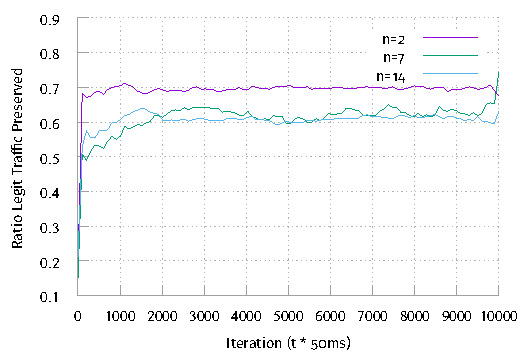
\includegraphics[width=\linewidth]{../plots/online-pres.pdf}
			\caption{Service quality decreases as actions become less granular.}
		\end{figure}
	\end{column}
	\end{columns}
\end{frame}

\section{The adversarial setting}

\begin{frame}{Attacks}
	\begin{description}
		\item[Poisoning attacks] Affect the training of a continuously learning model (RL agents, collaborative learning).
		
		\item[Evasion attacks] Make data/state appear to be different. These are what are often known as \alert{adversarial examples}!
	\end{description}
\end{frame}

\begin{frame}{The capabilities of attackers}
	\begin{itemize}
		\item \emph{Polymorphic blending attacks} (i.e., evasion) on past models are known \alert{\NP-Complete} by reduction to (s)FSA\footcite{DBLP:conf/ccs/FoglaL06}.
	
		\item We have empirical bounds on the effectiveness of poisoning attacks wrt.\ what percentage of inbound traffic an attacker controls\footcite{DBLP:journals/jmlr/KloftL10}.
		
		\item Careless model exposure $\implies$ \alert{black-box model extraction}\footcite{DBLP:conf/uss/TramerZJRR16} $\implies$ evasion\footcite{DBLP:conf/sp/Carlini017}.
		
		%\item Promising work on defences\footcite{DBLP:conf/acsac/CaoG17}.
	\end{itemize}
\end{frame}

\begin{frame}{Unknowns}
	\begin{itemize}
		\item We don't have results for poisoning on e.g., Deep RL in the network.
		\begin{itemize}
			\item Can an adversary precisely affect state at all measurement points?
			% Networks are unstable ``bursty'', and attacker has limited control over inbound traffic.
		\end{itemize}
		
		\item We also lack results on whether evasion attacks can transfer between policies which evolve over time.
		\begin{itemize}
			\item E.g., $\pi_t$ to $\pi_{t+\delta}$ for reinforcement learners focused on non-stationarity.
		\end{itemize}
		
	\end{itemize}
\end{frame}

\begin{frame}[standout]{Conclusion}
	We've looked at...
	\begin{itemize}
		\item A quick introduction to RL, and its \alert{importance to future networks}.
		\item A `direct control' approach to intrusion prevention, and \alert{intended improvements}.
		\item Adversarial work, security, and open questions.
	\end{itemize}
	
	\alert{Questions?}
\end{frame}

\appendix

\begin{frame}[allowframebreaks]{References}
\printbibliography[heading=none]
\end{frame}

\end{document}
